\documentclass{deliverablereport}

\usepackage[style=alphabetic,backend=bibtex]{biblatex}
\addbibresource{../../lib/kbibs/kwarcpubs.bib}
\addbibresource{../../lib/kbibs/extpubs.bib}
\addbibresource{../../lib/kbibs/kwarccrossrefs.bib}
\addbibresource{../../lib/kbibs/extcrossrefs.bib}
\addbibresource{../../lib/deliverables.bib}
%\addbibresource{../../lib/publications.bib}
\addbibresource{rest.bib}
% temporary fix due to http://tex.stackexchange.com/questions/311426/bibliography-error-use-of-blxbblverbaddi-doesnt-match-its-definition-ve
\makeatletter\def\blx@maxline{77}\makeatother

\usepackage{todonotes}

\deliverable{social-aspects}{social-datareport}
\deliverydate{02/28/2017}
\duedate{02/28/2017 (Month 18)}
\author{Dmitrii Pasechnik}

\begin{document}
\maketitle
%  Work Package WP6 develops a novel, foundational, knowledge-based framework for
  interfacing existing open source mathematical software systems and knowledge bases into
  a mathematical VRE, where systems can delegate functionalities among each other
  seamlessly without losing semantics.

  The overall Math-in-the-Middle (MitM) Framework developed in WP6 over the last three
  years is described in D6.5; this Report complements it by describing the curated
  contents Math-in-the-Middle (MitM) Ontology which serves as a reference and pivotal
  point for translations between the various input languages of mathematical software
  systems and knowledge bases.

  In a nutshell, the MitM Ontology describes the mathematical objects, concepts, and their
  relations in a general, system-agnostic way in an OMDoc/MMT theory graph while the
  mathematical systems export API theories that describe the system interface language in
  terms of types, classes, constructors, and functions -- again in OMDoc/MMT. These two
  levels of descriptions are linked by OMDoc/MMT alignments that allow the translation of
  expressions between systems.

%%% Local Variables:
%%% mode: visual-line
%%% fill-column: 5000
%%% mode: latex 
%%% TeX-master: "report"
%%% End:

\strut\githubissuedescription
\newpage\tableofcontents

\section{Questions and objectives}

Large-scale and to a lesser extent medium-scale open-source software 
is, as a rule, a product of a collaborative effort spanning many years of
development, improvements, bug fixes, ports to new platforms,
and partial or even full rewrites. A number of interesting related questions
arise in this context.
\begin{enumerate}
\item What are available data, measurement parameters and tools
allowing for analysis?
\item Can one assess the usefulness of the project by estimating
how ``alive'' it is, i.e. how much it is changing over time?
\item Can one reliably rank the contributors
by the effort put into the project?
\item Can one produce recommendations on the team size and composition
to ensure project's well-being?
\item Does the ``openness'' of the project matter?
\item Reliability of the system, stability of APIs etc., 
reproducibility of computational results, etc.
\end{enumerate}

\section{Data, parameters, and tools}

The main sources of information about the history of a project are versions of
its source code and records of various relevant communications, discussions, and
test results.  Before the wide acceptance of {\em revision control systems} 
(RCS) \cite{OSullivan:MakingSenseOfRCS} such as  CVS \cite{CVSWeb} and
Git \cite{ChaStr:pg14} the only readily available source code data came from
regular (often infrequent) public releases. Then it has become
more and more widespread, although not universal (cf. e.g. GAP \cite{gap},
which only in the past few years made its RCS 
public---and has not released earlier RCS data)
to keep the RCS {\em trees} holding {\em commits}---code changes
accompanied by comments---available online with read access for the public.

Communications on the project take basically three (not totally disjoint)
forms: mailing lists/bulletin
boards and tracker/code reviewing systems,
such as Trac \cite{wp7:trac}, Redmine \cite{wp7:redmine},
GitHub \cite{wp7:github},
Bitbucket \cite{wp7:bitbucket}, Gitlab \cite{wp7:gitlab},
etc, and documentation
systems/wikis. The latter is open by nature, whereas for the first two
the prevailing trend for these, at least in the domain related to the
ODK themes, is the ever increased
openness of the development process.

The current prevailing form of the analysis of the source code is based on
analysing authorship, frequency, and other parameters of commits in the RCS.
Most of the tools are in one or another way related to GitHub and its APIs to
access RCS trees and collect statistics, see e.g. \cite{wp7:arfonshapeoss}.
A sample of data obtained by such analysis may be found in Appendix below.
Communications are analysed using various text mining and analysis tools, such
as FOSS Heartbeat \cite{wp7:fossheartbeat}; these are not dissimilar to tools
used to analyse {\em social networks} such as Facebook
\cite{wp7:russell2013mining}.  Interestingly, GitHub as a collaborative social
network has been analysed \cite{wp7:githubandsof, DBLP:journals/corr/LimaRM14,
DBLP:journals/corr/VasilescuSWSB15, wp7:Kalliamvakou:2014:PPM:2597073.2597074}
and compared to Stack Overflow \cite{wp7:stackoverflow}. Note that analysis of
Mathoverflow (a sub-site of the latter) in \cite{MarPea:wmtapm13} was one of
the starting points in adding WP7 into the ODK project.

\section{Alive or dead? (Cathedral or Bazaar?)}
It is not obvious whether extreme stability of the code base,
such as e.g. Knuth's \TeX \cite{Knuth:ttb84}, with releases
numbered by consecutive digits of $\pi$, and only occurring
once every 5 or 6 years, see
\url{http://tug.org/texlive/devsrc/Build/source/texk/web2c/tex.web}
is a bad sign.
Although actively developed OSS projects are certainly showing 
a different pattern, with dozens of commits per day, etc., see
e.g. Figure~\ref{wp7:figsageadddel}. At this scale the dynamics of
the code of \TeX\ will be basically null.
\begin{figure}[ht]
  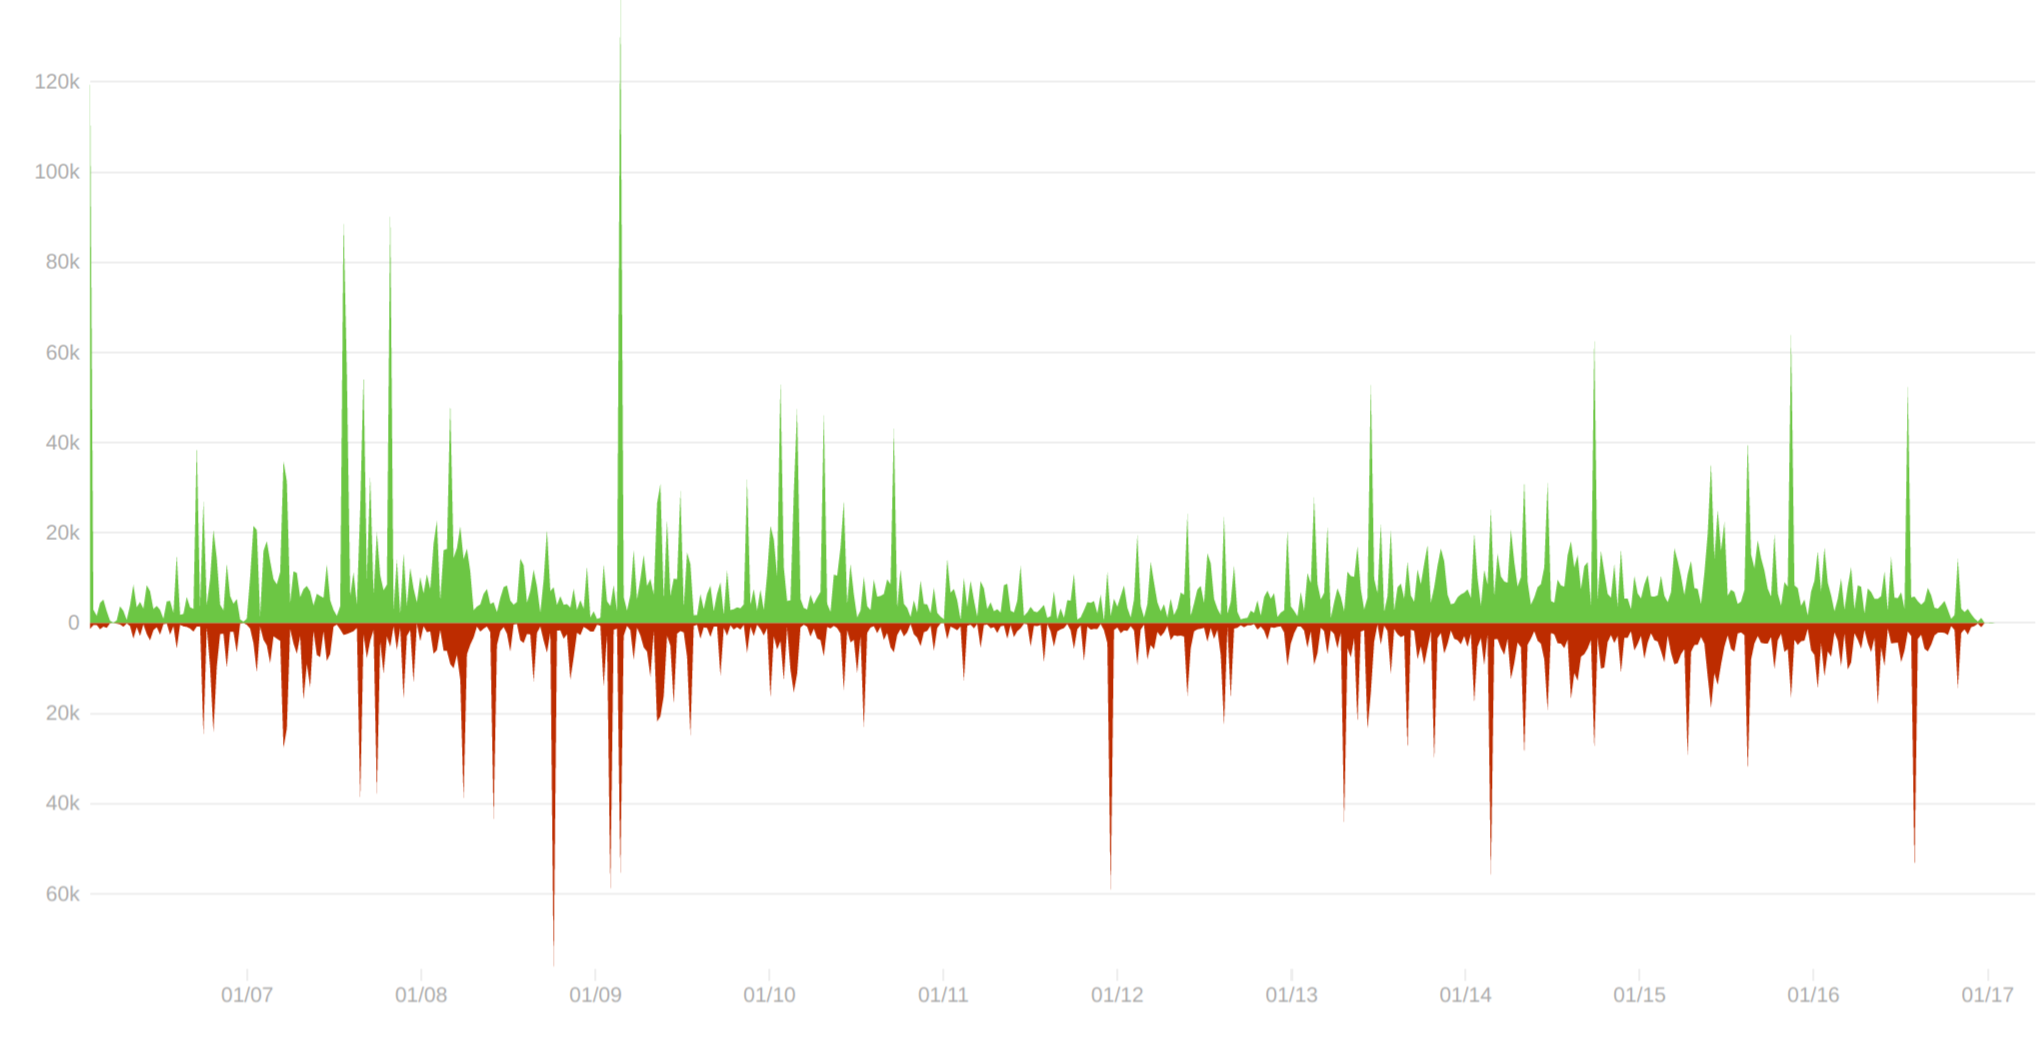
\includegraphics[width=\textwidth]{codeadddel}
    \caption{Code additions and deletions per week for 
    SageMath.\label{wp7:figsageadddel}}
\end{figure}
Different projects have vastly different cultures in regard of
commit frequency, commit size, etc., and this makes them 
hard to compare---something already observed in 
 \cite{raymond99:cathedral-bazaar}. 


\section{Ranking contributors}
This information may be extractable from a number of sources---
and headhunters for hi-tech companies publish guides on
how to utilise these for the search of talented software developers, cf.
e.g. \cite{wp7:sota}.

\subsection{Commits}
Are commits, as advocated by GitHub, a good way to rank contributors by their
contributions? Indeed, for GitHub, it is very easy to analyse the commits' (meta)data, computing the size of additions and deletions done by the commit,
and not so, as soon as real contributions are involved. To give one a simple example, how does
one measure the work done by quality assurance team, or by someone who does complicated debugging
and reports its results? Such an activity, if measured in commits, would fall under the radar almost
completely. As well, in some projects commits are squashed by release
managers, making them disappear all together.

There is also a lot of discrepancy between the commits in the
master branch (i.e. released versions) and the development branches---
people involved in making releases have more commits in the master
branch of mostly administrative kind, and they can be massive in size.

Bug fixing commits are often very short, although might be extremely
time consuming to create, compared to adding new code/documentation
and unit tests.


\subsection{Trackers and other exchanges}\label{wp7:sect:sentana}
Communications between developers, and to almost the same extent,
between users, and between users and developers, is an immense
source of information on the state of the project.
However, it is often a very loosely coupled textual data spread
over a range of different forms and mailing lists, and analysing it
needs text-mining tools. More structured data like this is available
on various issue/bug trackers. Still, it needs textological analysis for
sentiment. Experiments of this kind are known, cf. e.g.
\cite{wp7:fossheartbeat}, where analysis of OSS projects on parameters
like negative/positive sentiment in communication, friendliness of the
community towards the newcomers, etc., is analysed from the data
mined from GitHub, specifically from issue trackers and 
{\em pull requests} (i.e. patches proposed for the system, often by
external contributors).

An interesting option, not really explored so far, would be 
ranking issues by their importance, akin to the Stack Overflow
\cite{wp7:stackoverflow} sites.

\section{Team composition}
What is the optimal team composition for a successful OSS project?
Is the Cathedral model \cite{raymond99:cathedral-bazaar}
better or worse than the Bazaar one? It is hard to make a judgement on this,
as this heavily depends upon the application domain and the
size of the project. While our test computational system, \Sage
is developed very much in Bazaar style, many of its components
are pretty much Cathedral style ones.
Often it is possible to see just from the team size, which one is which.

What is clear from our experience is that it is very important
for the project to be open as long as bug tracking and pull requests
are concerned, while it's of secondary importance how exactly these are handled,
as long as they are handled within a reasonable time frame and in 
a respectful manner (users and potential contributors must be
respected).



\section{Openness, licensing, etc}

We will not argue here about the benefits of being open source for a
system, and only remark that this was validated not only empirically,
but by looking at the various growth rates before and after
open-sourcing, see e.g. \cite{wp7:arfonshapeoss}.


GPL and GPL-style licenses \cite{wp7:gpl} are often criticised for being
inflexible, too restrictive, etc., compared to less restrictive BSD-like
licenses. However, there is good evidence
to them being better in sense of keeping the community together. This can be
seen e.g. by noting how many forks of the BSD OS are out there
(dozens, including e.g. Apple's macOS, see
\cite{wp7:bsdlist}) and how many forks of Linux are out there
(none, essentially). 

\section{Reliability, stability of APIs, reproducibility}
Whenever a new external component is to be added to an OSS system,
a number of questions arise that can potentially be amenable to study through the
analysis of the flow of code and patches in the component.

Information on the reliability (i.e. how often critical level
bugs pop up, etc) of the system might be obtained from the issue/bug
trackers and from user forums and mailing lists, as well as from project's
announcements. However it does not look feasible to hope that
humans may be replaced, or even helped by, automatic tools to
make conclusions about the quality.

Application programming interfaces (APIs) are extremely
important parts of large-scale software systems.
A very important question is of {\em stability} of APIs, that is,
whether the API was in place for some time already and did not change
for a period of time---otherwise it might happen that a change in APIs will
require a redesign of the OSS.
While some APIs are extremely stable, e.g. famous BLAS's and LAPACK's
\cite{2002:USB:567806.567807,Anderson:1990:LPL:110382.110385}
APIs for numerical linear algebra, it is much less certain in more
modern areas, such as GPU computing, web programming, etc.

In the case of systems making regular (and well-documented)
releases it is normally possible to check stability of APIs
directly from the documentation. However it is becoming more and
more usual that there are no releases as such, the most fresh
``master branch'' of the RCS tree of the system is all that
can be taken as the release (essentially, the commit
hash has to be used to give the release a version number).
A slightly better situation is where ``stable'' releases are tagged
in the RCS with a version number label.
In these cases one could check the history of certain pieces
of the code in the RCS manually; however it might be 
desirable to have automated tools for this. Literature search for
the latter did not return anything that does not require
actual installation of the software in question and testing its APIs.




\section{Conclusions and future work}
A wide range of tools to pick up the low-hanging fruit--- 
the commit history from the RCS and project communications---
and study it are already available and can be readily applied
to open-source VREs and to their components.
However, it is unclear whether any practically interesting conclusions
and recommendations can be derived from such studies---not
the least due to their extreme imperfections discussed above.
One notable exception might be community sentiment analysis,
as discussed in Section~\ref{wp7:sect:sentana}. The latter is only
applicable to projects fully hosted on GitHub. While it might be
feasible to extend it to other development workflows, e.g. ones
using \cite{wp7:trac}, it appears to be out of scope of ODK.

Better mathematical models to analyse OSS ought to be developed, perhaps
by treating them as large-scale discrete dynamical systems
\cite{Antoulas:2005:ALD:1088857,Minati:2011:MMS:2208175}---whether
this is feasible is open to discussion.

\newpage

\section*{Appendix}
Here we include a sample of statistical data that can be obtained
for OSS projects, parts of \Sage fully hosted on GitHub.
We used \cite{wp7:fossheartbeat} to mine and process data
from the latter.

\subsection*{Some GAP statistics}
Figure \ref{wp7:fig:GAPissues} illustrates issue reporting
per contributor.
Currently most active, in these terms,
for the reported period, contributors, {\tt @alex-konovalov},
{\tt @fingolfin}, {\tt @markuspf}, and {\tt @ChrisJefferson}, 
correspond to the four top right points on the graph. 
Figure \ref{wp7:fig:GAPpulls} illustrates how fast pull
requests are dealt with.

\begin{figure}[ht]
  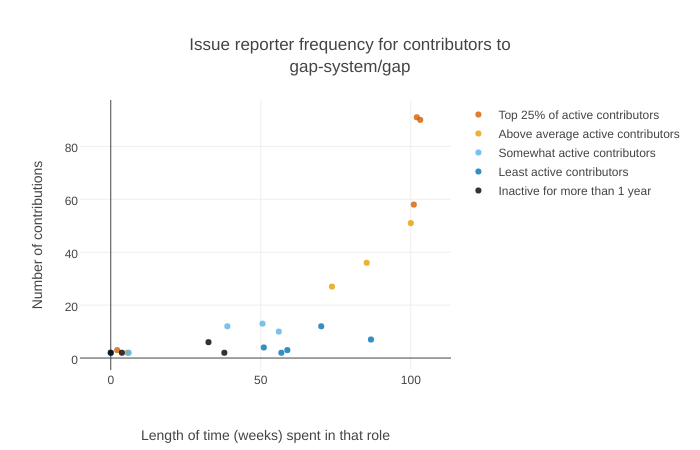
\includegraphics[width=\textwidth]{gap-issuereporting}
    \caption{Issues reporting for GAP.
    \label{wp7:fig:GAPissues}}
\end{figure}

\begin{figure}[ht]
  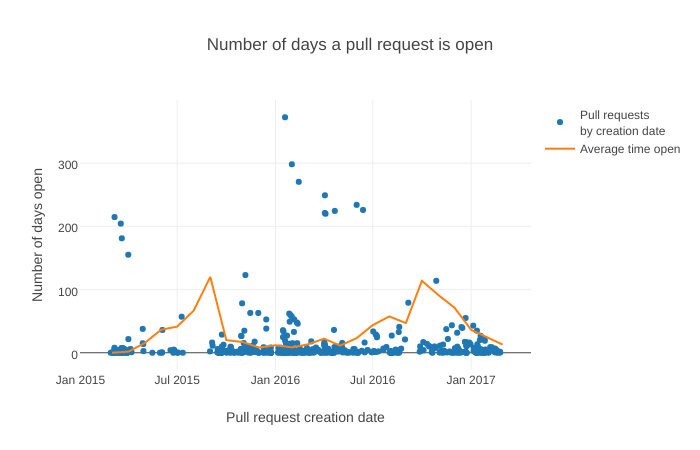
\includegraphics[width=\textwidth]{gap-pullrequests}
    \caption{Pull requests handling in GAP.\label{wp7:fig:GAPpulls}}
\end{figure}


\subsection*{Some SymPy statistics}
Figure \ref{wp7:fig:sympyissues} illustrates issue reporting
per contributor.
Currently most active, in these terms,
for the reported period, contributors, {\tt @certik} and {\tt @asmeuer}, 
correspond to the two top points on the graph. 

Figure \ref{wp7:fig:sympypulls} illustrates how fast pull
requests are dealt with.

\begin{figure}[ht]
  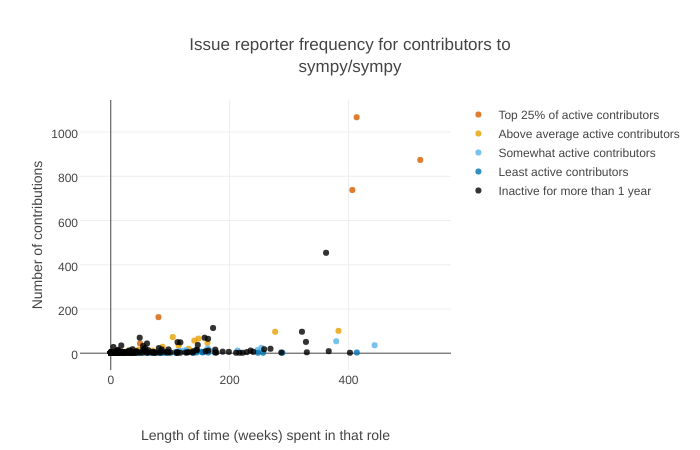
\includegraphics[width=\textwidth]{sympy-issuereporting}
    \caption{Issues reporting for SymPy. 
    \label{wp7:fig:sympyissues}}
\end{figure}

\begin{figure}[ht]
  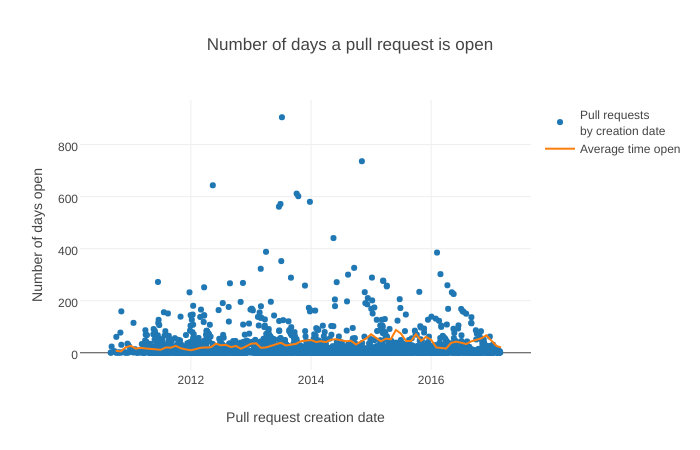
\includegraphics[width=\textwidth]{sympy-pullrequests}
    \caption{Pull requests handling in SymPy.\label{wp7:fig:sympypulls}}
\end{figure}

\newpage

\printbibliography
\end{document}

%%% Local Variables:
%%% mode: latex
%%% TeX-master: t
%%% End:

%  LocalWords:  githubissuedescription newpage tableofcontents newpage printbibliography
